\documentclass{jsreport}
\usepackage{graphicx, url, algorithm, algorithmic, float, booktabs, listings, color, pdfpages, amsmath, amssymb, latexsym, mathtools, ascmac, amsfonts, amsthm}
\lstset{
  basicstyle={\ttfamily},
  identifierstyle={\small},
  commentstyle={\smallitshape},
  keywordstyle={\small\bfseries},
  ndkeywordstyle={\small},
  stringstyle={\small\ttfamily},
  frame={tb},
  breaklines=true,
  columns=[l]{fullflexible},
  numbers=left,
  xrightmargin=0zw,
  xleftmargin=3zw,
  numberstyle={\scriptsize},
  stepnumber=1,
  numbersep=1zw,
  lineskip=-0.5ex
}
\usepackage[table,xcdraw]{xcolor}
\newtheorem{theo}{定理}[chapter]
\newtheorem{defi}{定義}[chapter]
\newtheorem{lemm}{補題}[chapter]
\newtheorem{prop}{命題}[chapter]
\newtheorem{coro}{系}[chapter]
\newcommand{\red}[1]{\textcolor{red}{#1}}
\newcommand{\blue}[1]{\textcolor{blue}{#1}}
\newcommand{\green}[1]{\textcolor{green}{#1}}
\renewcommand{\baselinestretch}{1.1}
\usepackage{mathrsfs}
\usepackage{bm}
\def\qed{\hfill $\Box$}
\usepackage{tikz}
\usetikzlibrary{intersections, calc, arrows}
\renewcommand\proofname{\bf 証明}

\begin{document}

\chapter{非線形計画問題}
本章では,非線形計画問題の最適性条件について述べる.

非線形計画問題においては,最適性の定義を次のように緩めることが多い.
\begin{itemize}
  \item $\bm{x}^*$は局所最小解(locally minimal solution)である.
  \begin{itemize}
    \item $\bm{x}^* \in S$に対し,ある近傍$B$が存在し,任意の$\bm{x} \in S \cap B$に対して$f(\bm{x}^*) \leq f(\bm{x})$が成立する.
  \end{itemize}
  \item $\bm{x}^*$は局所最大解(locally maximum solution)である.
  \begin{itemize}
    \item $\bm{x}^* \in S$に対し,ある近傍$B$が存在し,任意の$\bm{x} \in S \cap B$に対して$f(\bm{x}^*) \geq f(\bm{x})$が成立する.
  \end{itemize}
\end{itemize}

ここでは,最小化問題を基本としているので,局所最小解を局所最適解(locally optimal solution)ともいう.また,本来の最適解を大域最適解(globally optimal solution)という.
まず,局所最適解の必要条件,十分条件について述べ,局所最適解が大域最適解になる場合について述べる.

\section{制約なし問題の最適性条件}
本節では最適化問題として,(\ref{eq:opt_nonl_nonc})を考える.
\begin{align}\label{eq:opt_nonl_nonc}
  \mathrm{minimize} \; \; &f(\bm{x}) \nonumber\\
  \mathrm{subject \; to} \; \; &\bm{x} \in \mathbb{R}^n
\end{align}
ただし,$f$は任意の非線形関数であり,適当な微分可能性を仮定する.

問題(\ref{eq:opt_nonl_nonc})の最適性の必要条件として,次の2つの定理を示す.
\begin{theo}\label{theo:opt_nonl_nonc_h_1}
  $f \in C^{1}$のとき,$\bar{\bm{x}} \in \mathbb{R}^n$が問題(\ref{eq:opt_nonl_nonc})の局所最適解であるための必要条件は,
  \begin{equation}
    \nabla f(\bar{\bm{x}}) = \bm{0} \nonumber
  \end{equation}
  となることである.
\end{theo}

\begin{theo}\label{theo:opt_nonl_nonc_h_2}
  $f \in C^2$のとき,$\bar{\bm{x}}$が問題(\ref{eq:opt_nonl_nonc})の局所最適解であるための必要条件は,
  \begin{equation}
    \nabla f(\bar{\bm{x}}) = \bm{0} \nonumber
  \end{equation}
  かつ,$\bar{\bm{x}}$におけるヘッセ行列$H(\bar{\bm{x}})$が半正定値,すなわち,
  \begin{equation}
    \bm{d}^{\mathrm{T}} H(\bar{\bm{x}}) \bm{d} \geq 0, \; \forall \bm{d} \in \mathbb{R}^n \nonumber
  \end{equation}
  が成立することである.
\end{theo}

さらに,局所最適解の十分条件は,定理\ref{theo:opt_nonl_nonc_j}で与えられる.
\begin{theo}\label{theo:opt_nonl_nonc_j}
  $f \in C^2$のとき,$\bar{\bm{x}}$が問題(\ref{eq:opt_nonl_nonc})の局所最適解であるための十分条件は,
  \begin{equation}
    \nabla f(\bar{\bm{x}}) = \bm{0} \nonumber
  \end{equation}
  かつヘッセ行列$H(\bar{\bm{x}})$が正定値,すなわち,
  \begin{equation}
    \bm{d}^{\mathrm{T}} H(\bar{\bm{x}}) \bm{d} > 0, \; \forall \bm{d} \in \mathbb{R}^n, \; \bm{d} \neq \bm{0} \nonumber
  \end{equation}
  が成立することである.
\end{theo}

ここで,次の例題を解く.
\begin{align}\label{eq:opt_nonl_nonc}
  \mathrm{minimize} &: f(\bm{x}) = 2x_1^2 + x_1 x_2 + x_2^2 - 5x_1 - 3x_2 + 4 \nonumber\\
  \mathrm{subject \; to} &: \bm{x} \in \mathbb{R}^2 \nonumber
\end{align}
勾配ベクトルは,$\nabla f(\bm{x}) = (4x_1 + x_2 - 5, x_1 + 2x_2 - 3)^{\mathrm{T}}$であるので,$f$の停留点は,$x_1 = 1, x_2 = 1$である.また,$f$のヘッセ行列は,
\begin{equation}
  H(\bm{x}) = \left(
  \begin{array}{cc}
    4 & 1 \\
    1 & 2
  \end{array}
  \right) \nonumber
\end{equation}
であり,固有値$\lambda_1 = 3 + \sqrt{2}, \lambda_2 = 3 - \sqrt{2}$がともに正より,正定値である.よって,定理\ref{theo:opt_nonl_nonc_j}よりこの停留点は局所最適解である\footnote{$f$の等高線は,停留点を中心とした,2軸が固有ベクトルの楕円となる.}.\qed

\section{等式制約問題の最適性条件}
本節では最適化問題として,(\ref{eq:opt_nonl_eq})を考える.
\begin{align}\label{eq:opt_nonl_eq}
  \mathrm{minimize} \; \; &f(\bm{x}) \nonumber\\
  \mathrm{subject \; to} \; \; &g_i(\bm{x}) = 0, \; i = 1, 2, \ldots, m \nonumber \\
  &\bm{x} \in \mathbb{R}^n
\end{align}

等式制約問題(\ref{eq:opt_nonl_eq})における主要な結果は,目的関数$f(\bm{x})$の代わりにLagrange関数(Lagrangian function)
\begin{equation}\label{eq:lag}
  L(\bm{x}, \bm{u}) = f(\bm{x}) + \bm{u}^{\mathrm{T}} \bm{g}(\bm{x})
\end{equation}
を用いると,前節の定理\ref{theo:opt_nonl_nonc_h_1},定理\ref{theo:opt_nonl_nonc_h_2}を自然に拡張できるという点にある.
ただし,$\bm{u} \in \mathbb{R}^m, \, \bm{g}(\bm{x}) = (g_1(\bm{x}), g_2(\bm{x}), \ldots, g_m(\bm{x}))^{\mathrm{T}}$である.

\paragraph{等式条件のペナルティ関数}
問題(\ref{eq:opt_nonl_eq})とパラメータ$k = 1, 2, \ldots$から次の関数を定義する.
\begin{equation}\label{eq:penalty}
  F^k(\bm{x}) = f(\bm{x}) + \frac{k}{2}\|\bm{g}(\bm{x})\|^2 + \frac{\alpha}{2}\|\bm{x} - \bar{\bm{x}}\|^2
\end{equation}
ただし,$\bar{\bm{x}}$は,問題(\ref{eq:opt_nonl_eq})の局所最適解である.また,$\alpha > 0$
とする.
(\ref{eq:penalty})式において,第2項は,等式制約の違反に対するペナルティと解釈することができる.第3項は,$\bm{g}(\bm{x}) = \bm{0}$を満たす解$\bm{x}$を考えるとき,$\bar{\bm{x}}$が近傍内で$F^k(\bm{x})$の唯一の局所最適解となるように導入されたものである.

$\bar{\bm{x}}$は局所最適解であるので,適当な$\varepsilon > 0$を選べば,$\bar{\bm{x}}$の近傍の閉包
\begin{equation}
  \bar{B}(\bar{\bm{x}}, \varepsilon) = \{\bm{x} \in \mathbb{R}^n \, | \, \|\bm{x} - \bar{\bm{x}}\| \leq \varepsilon\}
\end{equation}
において,そこに属す任意の実行可能解$\bm{x}$に対して,$f(\bar{\bm{x}}) \leq f(\bm{x})$である最適化問題
\begin{align}\label{eq:opt_penal}
  \mathrm{minimize} \; \; &F^k(\bm{x}) \nonumber\\
  \mathrm{subject \; to} \; \; &\bm{x} \in \bar{B}(\bar{\bm{x}}, \varepsilon)
\end{align}
を定義する.$\bar{B}(\bar{\bm{x}}, \varepsilon)$は有界閉集合より,Weierstrassの定理から最小解が存在する.
最小解$\bm{x}^k$による点列$\{\bm{x}^k\}$が$\bar{\bm{x}}$に収束することを示す.

任意の$k$に対し,$\bm{x}^k$の最適性より,
\begin{align}\label{eq:opt_penal_cond}
  F^k(\bm{x}^k) &= f(\bm{x}^k) + \frac{k}{2}\|g(\bm{x}^k)\|^2 + \frac{\alpha}{2}\|\bm{x}^k - \bar{\bm{x}}\|^2 \nonumber \\
  &\leq F^k(\bar{\bm{x}}) = f(\bar{\bm{x}})
\end{align}
より,$\lim \limits_{k \rightarrow \infty} \|\bm{g}(\bm{x}^k)\| = 0$でなければならない\footnote{これを満たさなければ,$k \rightarrow \infty$で発散する.}.
従って,$\{\bm{x}^k\}$の任意の極限点$\bar{\bar{\bm{x}}}$は,$\bm{g}(\bar{\bar{\bm{x}}}) = 0$を満たすので,最適化問題(\ref{eq:opt_nonl_eq})の実行可能解である.
(\ref{eq:opt_penal_cond})式から,
\begin{equation}
  f(\bar{\bar{\bm{x}}}) + \frac{\alpha}{2}\|\bar{\bar{\bm{x}}} - \bar{\bm{x}}\|^2 \leq f(\bar{\bm{x}}) \nonumber
\end{equation}
を得る.また,$\bar{\bar{\bm{x}}}$が,元の問題(\ref{eq:opt_nonl_eq})の実行可能解であることから,
$f(\bar{\bm{x}}) \leq f(\bar{\bar{\bm{x}}})$.これと上式を合わせて,
\begin{equation}
  \|\bar{\bar{\bm{x}}} - \bar{\bm{x}}\|^2 = 0 \; \therefore \bar{\bar{\bm{x}}} = \bar{\bm{x}} \nonumber
\end{equation}

つまり,点列$\{\bm{x}^k\}$は$\bar{\bm{x}}$に収束する.点$\bar{\bm{x}}$は問題(\ref{eq:opt_penal})の実行可能領域の内点である.また,$k$が十分大きければ,$\bm{x}^k$も内点である.
したがって,$\bm{x}^k$は制約なしの最適化問題
\begin{align}\label{eq:opt_penal_non}
  \mathrm{minimize} &: F^k(\bm{x}) \nonumber\\
  \mathrm{subject \; to} &: \bm{x} \in \mathbb{R}^n
\end{align}
の局所最適解でもある.

\paragraph{等式制約問題の最適性必要条件}
問題(\ref{eq:opt_nonl_eq})の$m$個の制約関数の勾配ベクトル$g_i(\bm{x}), \, i = 1, 2, \ldots, m$が互いに線形独立であるとき,点$\bm{x}$は正則(regular)であるという.
問題(\ref{eq:opt_nonl_eq})の最適性の必要条件は,定理\ref{theo:opt_nonl_eq_h}で与えられる.
\begin{theo}\label{theo:opt_nonl_eq_h}
  \begin{enumerate}
    \item 1次の最適性必要条件\label{enu:1}

    $f, g_i \in C^1, \, i = 1, 2, \ldots, m$であり,$\bar{\bm{x}}$が正則であるとき,$\bar{\bm{x}} \in \mathbb{R}^n$が問題(\ref{eq:opt_nonl_eq})の局所最適解であるための必要条件は,
    \begin{equation}\label{eq:opt_nonl_eq_h_1}
      \nabla f(\bar{\bm{x}}) + \sum_{i = 1}^m u_i \nabla g_i(\bar{\bm{x}}) = \bm{0}
    \end{equation}
    を満たすラグランジュ乗数ベクトル$\bm{u} = (u_1, u_2, \ldots, u_m)^{\mathrm{T}}$が存在することである\footnote{ラグランジュ乗数ベクトル$\bm{u}$は,等式制約条件の右辺の変化が目的関数値にどのような影響を持つかを示すベクトルである.}.

    \item 2次の最適性必要条件

    \ref{enu:1}の仮定に加え,$f, g_i \in C^2, \, i = 1, 2, \ldots, m$であるとき,
    $\bar{\bm{x}} \in \mathbb{R}^n$が問題(\ref{eq:opt_nonl_eq})の局所最適解であるための必要条件は,
    \begin{align}\label{eq:opt_nonl_eq_h_2}
      &\nabla f(\bar{\bm{x}}) + \sum_{i = 1}^m u_i \nabla g_i(\bar{\bm{x}}) = \bm{0} \nonumber \\
      &\bm{y}^{\mathrm{T}} \left({\nabla}^2 f(\bar{\bm{x}}) + \sum_{i = 1}^m u_i {\nabla}^2 g_i(\bar{\bm{x}})\right) \bm{y} \geq 0, \; \forall \bm{y} \in V(\bar{\bm{x}})
    \end{align}
    を満たすラグランジュ乗数ベクトル$\bm{u} = (u_1, u_2, \ldots, u_m)^{\mathrm{T}}$が存在することである.ただし,
    \begin{equation}\label{eq:v}
      V(\bar{\bm{x}}) = \{\bm{y} \in \mathbb{R}^n \, | \, \nabla \bm{g}(\bar{\bm{x}}) \bm{y} = \bm{0}\}
    \end{equation}
    である.
  \end{enumerate}
\end{theo}

ここで,Lagrange関数(\ref{eq:lag})を用いると,等式制約条件$\bm{g}(\bm{x}) = 0$および条件(\ref{eq:opt_nonl_eq_h_1}),(\ref{eq:opt_nonl_eq_h_2})は次のように表される.
\begin{align}
  &\nabla_{\bm{u}} L(\bar{\bm{x}}, \bm{u}) = \bm{0} \nonumber \\
  &\nabla_{\bm{x}} L(\bar{\bm{x}}, \bm{u}) = \bm{0} \nonumber \\
  &\bm{y}^{\mathrm{T}} {\nabla}^2_{\bm{xx}} L(\bar{\bm{x}}, \bm{u}) \bm{y} \geq 0, \; \forall \bm{y} \in V(\bar{\bm{x}}) \nonumber
\end{align}

\paragraph{最適性条件の幾何学的解釈}
条件(\ref{eq:opt_nonl_eq_h_1})の幾何学的な意味を考察する.簡単のため,制約条件が1つの場合,すなわち,制約条件が$g(\bm{x}) = 0$の場合を考える.条件(\ref{eq:opt_nonl_eq_h_1})は,
$\nabla f(\bm{x}) + u \nabla g(\bm{x}) = 0$と書くことができる.$u$の符号をどちらにとっても良いことから,この条件は,2つのベクトル$\nabla f(\bm{x})$と$\nabla g(\bm{x})$が同方向か,あるいは逆方向であることを述べている.
$g(\bm{x}) = 0$の範囲内で微小量移動することは,$\nabla g(\bm{x})$の直交方向に進むことに相当する.この方向は$\nabla f(\bm{x})$とも直行しているので,目的関数値は変化せず,最適性の必要条件を与える.
複数の制約条件を持つ一般の場合,条件(\ref{eq:opt_nonl_eq_h_1})は,ベクトル$\nabla g_i(\bm{x}), \; i = 1, 2, \ldots, m$が張る空間内にベクトル$\nabla f(\bm{x})$が位置していることを要求している.これも上と同様の解釈が可能である.


\paragraph{等式制約問題の最適性十分条件}
制約なし問題の最適性の十分条件(定理\ref{theo:opt_nonl_nonc_j})を等式制約の場合へ拡張する.十分条件は,定理\ref{theo:opt_nonl_eq_j}で与えられる.
\begin{theo}\label{theo:opt_nonl_eq_j}
  $f, g_i \in C^2, \, i = 1, 2, \ldots, m$であるとき,
  $\bar{\bm{x}} \in \mathbb{R}^n$が問題(\ref{eq:opt_nonl_eq})の局所最適解であるための十分条件は,
  \begin{align}
    &\nabla_{\bm{u}} L(\bar{\bm{x}}, \bm{u}) = \bm{0} \nonumber \\
    &\nabla_{\bm{x}} L(\bar{\bm{x}}, \bm{u}) = \bm{0} \nonumber \\
    &\bm{y}^{\mathrm{T}} {\nabla}^2_{\bm{xx}} L(\bar{\bm{x}}, \bm{u}) \bm{y} > 0, \; \forall \bm{y}(\neq \bm{0}) \in V(\bar{\bm{x}}) \nonumber
  \end{align}
  を満たすラグランジュ乗数ベクトル$\bm{u} = (u_1, u_2, \ldots, u_m)^{\mathrm{T}}$が存在することである.
\end{theo}

ここで,次の例題を解く.
\begin{align}
  \mathrm{minimize} \; \; &f(\bm{x}) = -x_1 x_2 \nonumber\\
  \mathrm{subject \; to} \; \; &g(\bm{x}) = x_1^2 + x_2^2 - 1 = 0 \nonumber \\
  &\bm{x} \in \mathbb{R}^2 \nonumber
\end{align}
Lagrange関数を$L(\bm{x}, u)$とすると,
\begin{equation}
  L(\bm{x}, u) = f(\bm{x}) + u g(\bm{x}) = -x_1 x_2 + u(x_1^2 + x_2^2 - 1) \nonumber
\end{equation}
最適性の必要条件より,
\begin{align}
  &\nabla_u L(\bm{x}, u) = x_1^2 + x_2^2 - 1 = 0 \nonumber \\
  &\nabla_{\bm{x}} L(\bm{x}, u) = \left(
  \begin{array}{c}
    -x_2 \\
    -x_1
  \end{array}
  \right) + u\left(
  \begin{array}{c}
    2x_1 \\
    2x_2
  \end{array}
  \right) = \bm{0} \nonumber
\end{align}
この連立方程式を解くと,
\begin{equation}
  (\bar{x}_1, \bar{x}_2, u) =
  \left(\frac{1}{\sqrt{2}}, \frac{1}{\sqrt{2}}, \frac{1}{2}\right), \,
  \left(- \frac{1}{\sqrt{2}}, - \frac{1}{\sqrt{2}}, \frac{1}{2}\right), \,
  \left(\frac{1}{\sqrt{2}}, - \frac{1}{\sqrt{2}}, - \frac{1}{2}\right), \,
  \left(- \frac{1}{\sqrt{2}}, \frac{1}{\sqrt{2}}, - \frac{1}{2}\right) \nonumber
\end{equation}
が得られる.前半の2つの解について,
\begin{align}
  \nabla_{\bm{xx}} L(\bar{\bm{x}}, u) &= {\nabla}^2 f(\bar{\bm{x}}) + u {\nabla}^2 g(\bar{\bm{x}}) \nonumber \\
  &= \left(
  \begin{array}{cc}
    0 & -1 \\
    -1 & 0
  \end{array}
  \right) + \frac{1}{2} \left(
  \begin{array}{cc}
    2 & 0 \\
    0 & 2
  \end{array}
  \right) = \left(
  \begin{array}{cc}
    1 & -1 \\
    -1 & 1
  \end{array}
  \right) \nonumber
\end{align}
から,固有値$\lambda_1, \lambda_2$は,$\lambda_1 = 2, \lambda_2 = 0$.よって,この行列は半正定値であり,任意の$\bm{y}$に対し,$\bm{y}^{\mathrm{T}} (\nabla_{\bm{xx}}) \bm{y} \geq 0$を満たす.よって,この2解は最適性の必要条件を満たす.

次に,後半の2解についても同様に$\nabla_{\bm{xx}}$を求めると,
\begin{equation}
  \nabla_{\bm{xx}} = \left(
  \begin{array}{cc}
    -1 & -1 \\
    -1 & -1
  \end{array}
  \right) \nonumber
\end{equation}
から,固有値$\lambda_1, \lambda_2$は,$\lambda_1 = 0, \lambda_2 = -2$.よって,この行列は半負定値である.
2解に対し,$(\nabla g(\bar{\bm{x}}))^{\mathrm{T}} \bm{y} = \bm{0}$を満たすベクトル$y$の集合は,パラメータ$t$を用いて,
\begin{equation}
  V(\bar{\bm{x}}) = \{\bm{y} = (t, t)^{\mathrm{T}} \, | \, t \in \mathbb{R} \} \nonumber
\end{equation}
と書ける.これを用いると,
\begin{equation}
  \left(
  \begin{array}{cc}
    t & t
  \end{array}
  \right) \left(
  \begin{array}{cc}
    -1 & -1 \\
    -1 & -1
  \end{array}
  \right) \left(
  \begin{array}{c}
    t \\
    t
  \end{array}
  \right) = -4t^2 \nonumber
\end{equation}
である.これは,$t \neq 0$で負の値を取り,最適性の必要条件を満たさない.よって,この2解は局所最適解ではない.

必要条件を満たす2解に対して,$(\nabla g(\bar{\bm{x}}))^{\mathrm{T}} \bm{y} = \bm{0}$を満たすベクトル$y$の集合は,パラメータ$t$を用いて,
\begin{equation}
  V(\bar{\bm{x}}) = \{\bm{y} = (t, -t)^{\mathrm{T}} \, | \, t \in \mathbb{R} \} \nonumber
\end{equation}
である.よって,
\begin{equation}
  \left(
  \begin{array}{cc}
    t & -t
  \end{array}
  \right) \left(
  \begin{array}{cc}
    1 & -1 \\
    -1 & 1
  \end{array}
  \right) \left(
  \begin{array}{c}
    t \\
    -t
  \end{array}
  \right) = 4t^2 \geq 0 \nonumber
\end{equation}
であり,$t \neq 0$では正の値を取る.よって,これは最適性の十分条件を満たす.

以上より,この問題の局所最適解は,
\begin{equation}
  \bar{\bm{x}} = \left(\frac{1}{\sqrt{2}}, \frac{1}{\sqrt{2}}\right)^{\mathrm{T}}, \, \left(- \frac{1}{\sqrt{2}}, - \frac{1}{\sqrt{2}}\right)^{\mathrm{T}} \nonumber
\end{equation}
であり,その目的関数値は$-1/2$である.\qed

\section{不等式制約問題の最適性条件}
本節では最適化問題として,(\ref{eq:opt_nonl_f})を考える.
\begin{align}\label{eq:opt_nonl_f}
  \mathrm{minimize} \; \; &f(\bm{x}) \nonumber\\
  \mathrm{subject \; to} \; \; &g_i(\bm{x}) \leq 0, \; i = 1, 2, \ldots, l \nonumber \\
  &g_i(\bm{x}) = 0, \; i = l+1, \ldots, m \nonumber \\
  &\bm{x} \in \mathbb{R}^n
\end{align}
実行可能解$\bm{x}$は,各不等式条件$g_i(\bm{x}) = 0$を等式で満たす場合と真の不等式で満たす場合がある.不等式条件において,$g_i(\bm{x}) = 0$となるものを,$\bm{x}$において有効である(active)という.
有効制約条件の添字集合を,
\begin{equation}\label{eq:activesubscript}
  A(\bm{x}) = \{i \, | \, g_i(\bm{x}) = 0, \; i = 1, 2, \ldots, l\}
\end{equation}
と記す.実行可能解$\bm{x}$において,等式で成立する条件の勾配ベクトル$\nabla g_i(\bm{x}), \, i \in A(\bm{x})$および$\nabla g_i(\bm{x}), \, i = l + 1, \ldots, m$が線形独立であるとき,$\bm{x}$は正則(regular)であるという.

\paragraph{不等式制約問題の最適性条件}
Lagrange関数(\ref{eq:lag})に基づく等式制約問題の最適性条件(定理\ref{theo:opt_nonl_eq_h})の一般化を行う.
問題(\ref{eq:opt_nonl_f})の最適性の必要条件は,定理\ref{theo:opt_nonl_f_h}で与えられる.
\begin{theo}\label{theo:opt_nonl_f_h}
  \begin{enumerate}
    \item 1次の最適性必要条件\label{enu:f1}

    $f, g_i \in C^1, \, i = 1, 2, \ldots, m$であり,$\bar{\bm{x}}$が正則であるとき,$\bar{\bm{x}} \in \mathbb{R}^n$が問題(\ref{eq:opt_nonl_f})の局所最適解であるための必要条件は,
    \begin{align}\label{eq:opt_nonl_f_h}
      &\nabla_{\bm{x}} L(\bar{\bm{x}}, \bm{u}) = \nabla f(\bar{\bm{x}}) + \sum_{i = 1}^m u_i \nabla g_i(\bar{\bm{x}}) = \bm{0} \nonumber \\
      &u_i \geq 0, \; i = 1, 2, \ldots, l \nonumber \\
      &u_i = 0, \; i \in \{1, 2, \ldots, l\} - A(\bar{\bm{x}})
    \end{align}
    を満たすラグランジュ乗数ベクトル$\bm{u} \in \mathbb{R}^m$が存在することである\footnote{不等式制約のうち,有効でないものに対する$u_i$は$0$.等式制約の$u_i, \, i = l + 1, \ldots, m$に対する符号制約はない.}.

    \item 2次の最適性必要条件

    \ref{enu:f1}の仮定に加え,$f, g_i \in C^2, \, i = 1, 2, \ldots, m$であるとき,
    $\bar{\bm{x}} \in \mathbb{R}^n$が問題(\ref{eq:opt_nonl_f})の局所最適解であるための必要条件は,(\ref{eq:opt_nonl_f_h})に加え,
    \begin{align}\label{eq:opt_nonl_f_h_2}
      &\bm{y}^{\mathrm{T}} \left({\nabla}^2 f(\bar{\bm{x}}) + \sum_{i = 1}^m u_i {\nabla}^2 g_i(\bar{\bm{x}})\right) \bm{y} \geq 0, \; \forall \bm{y} \in V^{\prime}(\bar{\bm{x}})
    \end{align}
    を満たすラグランジュ乗数ベクトル$\bm{u} = (u_1, u_2, \ldots, u_m)^{\mathrm{T}}$が存在することである.ただし,
    \begin{equation}\label{eq:fv}
      V^{\prime}(\bar{\bm{x}}) = \{\bm{y} \in \mathbb{R}^n \, | \, \nabla g_i(\bar{\bm{x}})^{\mathrm{T}} \bm{y} = \bm{0}, \, i \in A(\bar{\bm{x}}) \cup \{l + 1, \ldots, m\} \}
    \end{equation}
    である.
  \end{enumerate}
\end{theo}

ここで,(\ref{eq:opt_nonl_f_h})の3番目の条件は,
\begin{equation}\label{eq:comp}
  u_i g_i(\bar{\bm{x}}) = 0, \; i = 1, 2, \ldots, l
\end{equation}
と書くことができる\footnote{$g_i(\bar{\bm{x}}) < 0$ならば$u_i = 0$,$g_i(\bar{\bm{x}}) = 0$ならば$u_i \geq 0$.}.この条件は相補性条件(complementarity condition)と呼ばれる.また,定理\ref{theo:opt_nonl_f_h}の式(\ref{eq:opt_nonl_f_h})および(\ref{eq:opt_nonl_f_h_2})はKKT条件と呼ばれている
\footnote{KKT条件は,$\bar{\bm{x}}$から実行可能領域のどの方向を選んでも,$-\nabla f(\bar{\bm{x}})$と鋭角をなすことができず,目的関数値を減少させることができないことを示している(後述).}.

\paragraph{不等式制約問題の最適性十分条件}
定理\ref{theo:opt_nonl_eq_j}にならって,不等式制約問題(\ref{eq:opt_nonl_f})に対する2次の最適性十分条件を与える.
\begin{theo}\label{theo:opt_nonl_f_j}
  $f, g_i \in C^2, \, i = 1, 2, \ldots, m$であるとき,
  $\bar{\bm{x}} \in \mathbb{R}^n$が問題(\ref{eq:opt_nonl_f})の局所最適解であるための十分条件は,

  \begin{align}
    &g_i(\bar{\bm{x}}) \leq 0, \; i = 1, 2, \ldots, l \nonumber \\
    &g_i(\bar{\bm{x}}) = 0, \; i = l + 1, \ldots, m \nonumber \\
    &\nabla f(\bar{\bm{x}}) + \sum_{i = 1}^m u_i \nabla g_i(\bar{\bm{x}}) = \bm{0} \nonumber \\
    &u_i > 0, \; i \in A(\bar{\bm{x}}) \nonumber \\
    &u_i = 0, \; i \in \{1, 2, \ldots, l\} - A(\bar{\bm{x}}) \nonumber \\
    &\bm{y}^{\mathrm{T}} \left({\nabla}^2 f(\bar{\bm{x}}) + \sum_{i = 1}^m u_i {\nabla}^2 g_i(\bar{\bm{x}})\right) \bm{y} > 0, \; \forall \bm{y}(\neq \bm{0}) \in V^{\prime}(\bar{\bm{x}})
  \end{align}
  を満たすラグランジュ乗数ベクトル$\bm{u} = (u_1, u_2, \ldots, u_m)^{\mathrm{T}}$が存在することである.
  ただし,$A(\bar{\bm{x}})$の定義は(\ref{eq:activesubscript})式,$V^{\prime}(\bar{\bm{x}})$の定義は(\ref{eq:fv})式にある.
\end{theo}

ここで,次の例題を解く.
\begin{align}
  \mathrm{minimize} \; \; &f(\bm{x}) = 2x_1^2 + x_1 x_2 + x_2^2 + x_1 - 3x_2 + 3 \nonumber\\
  \mathrm{subject \; to} \; \; &g_1(\bm{x}) = x_1^2 + x_2^2 - 1 \leq 0 \nonumber \\
  &g_2(\bm{x}) = -x_1 \leq 0 \nonumber \\
  &g_3(\bm{x}) = -x_2 \leq 0 \nonumber \\
  &\bm{x} \in \mathbb{R}^2 \nonumber
\end{align}

目的関数および制約式の勾配ベクトルはそれぞれ,
\begin{align}
  \nabla f(\bm{x}) &= (4x_1 + x_2 + 1, x_1 + 2x_2 - 3)^{\mathrm{T}} \nonumber \\
  \nabla g_1(\bm{x}) &= (2x_1, 2x_2)^{\mathrm{T}} \nonumber \\
  \nabla g_2(\bm{x}) &= (-1, 0)^{\mathrm{T}} \nonumber \\
  \nabla g_3(\bm{x}) &= (0, -1)^{\mathrm{T}} \nonumber
\end{align}
よって,$f$の停留点は,$(-5/7, 13/7)$である.また,$f$のヘッセ行列は,
\begin{equation}
  \nabla^2 f(\bm{x}) = \left(
  \begin{array}{cc}
    4 & 1 \\
    1 & 2
  \end{array}
  \right) \nonumber
\end{equation}
から,固有値は$\lambda_1 = 3 + \sqrt{2}, \lambda_2 = 3 - \sqrt{2}$であり,固有値$\lambda_1, \lambda_2$に属する固有ベクトルはそれぞれ$\bm{v}_1 = (1, \sqrt{2} - 1)^{\mathrm{T}}, \bm{v}_2 = (1, -\sqrt{2} - 1)^{\mathrm{T}}$である.
この問題の実行可能領域および$f$の等高線を図\ref{fig:feasible_f}に示す.
\begin{figure}[tb]
  \centering
  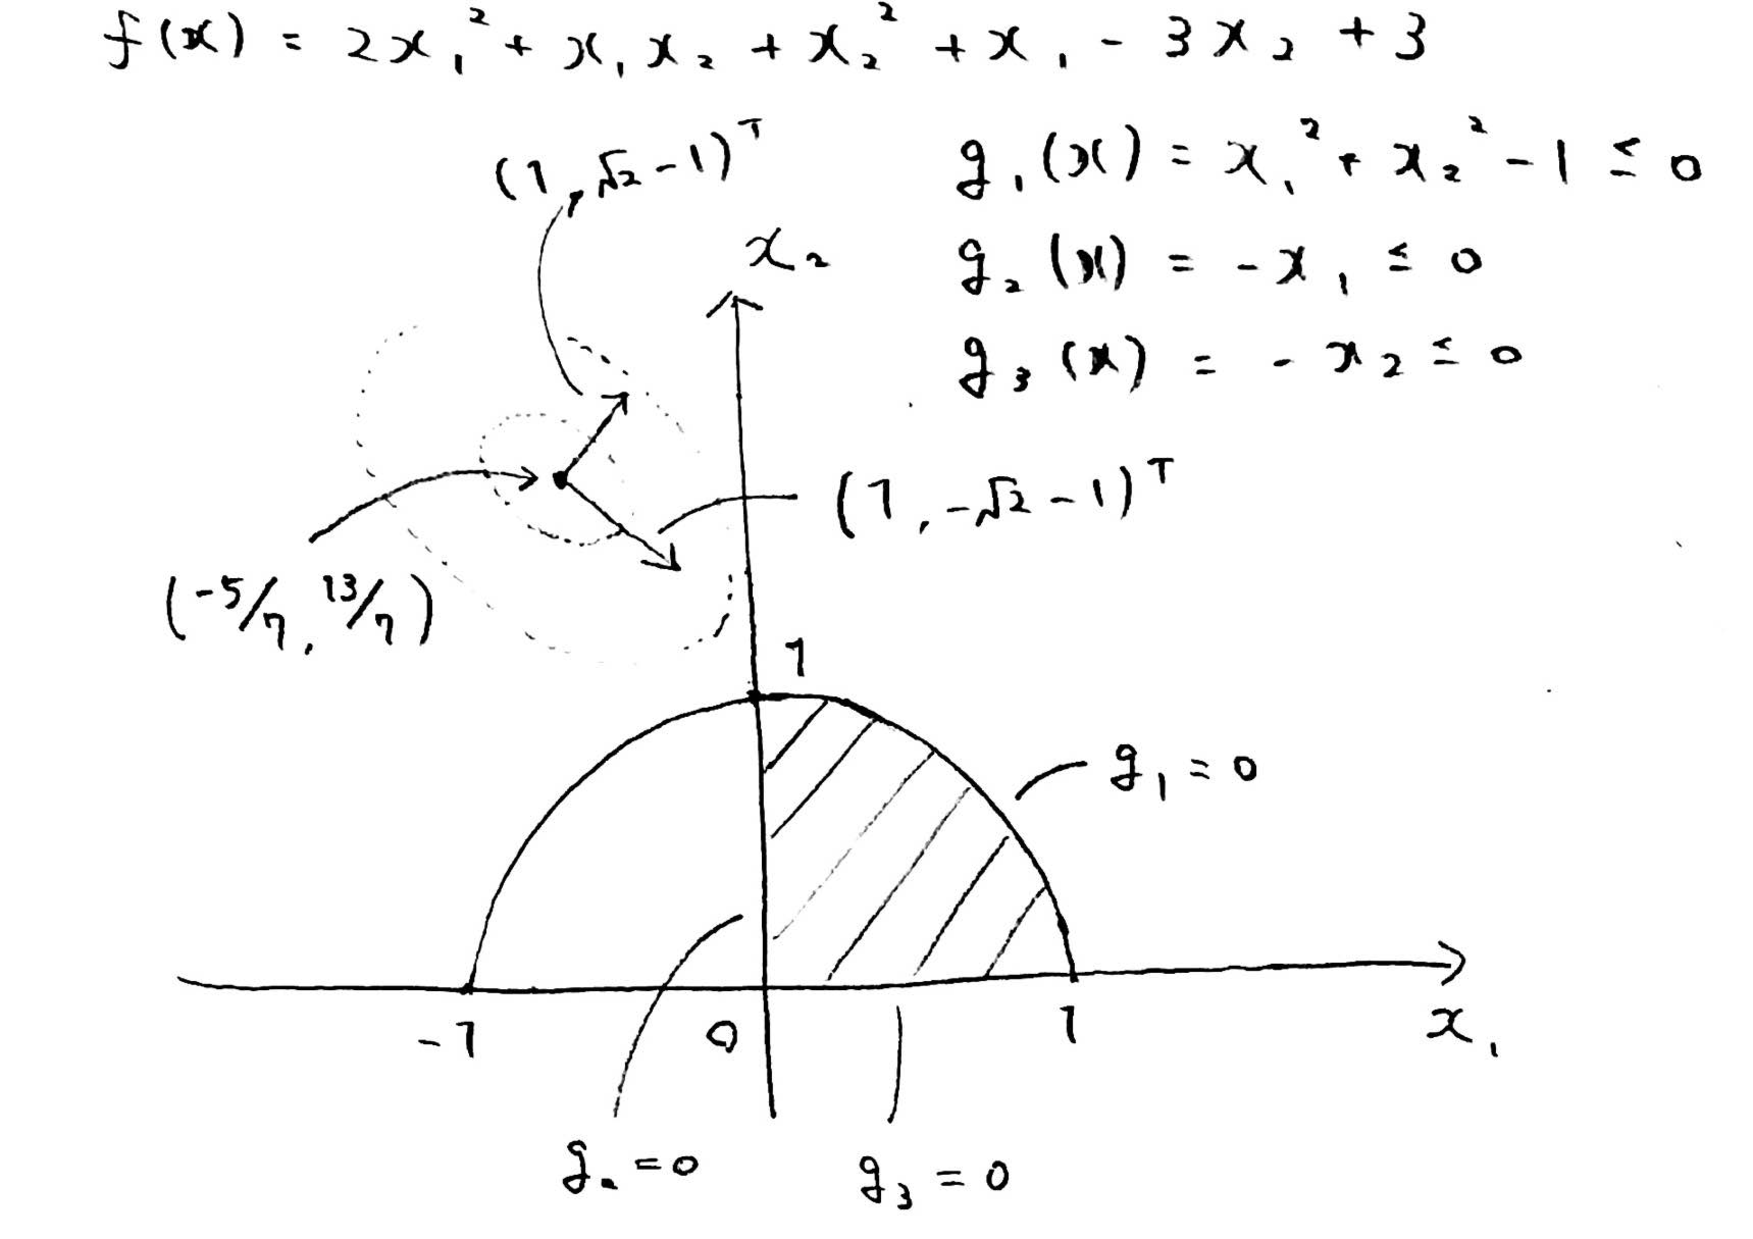
\includegraphics[clip, width=7cm]{../figure/KKT_1.pdf}
  \caption{実行可能領域と$f$の等高線}
  \label{fig:feasible_f}
\end{figure}

有効制約は$g_1(\bm{x}), g_2(\bm{x})$と考えられる.よって,
\begin{align}
  &\left(
  \begin{array}{c}
    4x_1 + x_2 + 1 \\
    x_1 + 2x_2 - 3
  \end{array}
  \right) + u_1\left(
  \begin{array}{c}
    2x_1 \\
    2x_2
  \end{array}
  \right) + u_2\left(
  \begin{array}{c}
    -1 \\
    0
  \end{array}
  \right) = \left(
  \begin{array}{c}
    0 \\
    0
  \end{array}
  \right) \nonumber \\
  &x_1^2 + x_2^2 - 1 = 0 \nonumber \\
  &-x_1 = 0 \nonumber \\
  &u_3 = 0 \nonumber
\end{align}
より,実行可能解で1次の最適性必要条件を満たすものは,
\begin{equation}
  (\bar{x}_1, \bar{x}_2, u_1, u_2) = \left(0, 1, \frac{1}{2}, 2 \right) \nonumber
\end{equation}
また,
\begin{equation}
  \left(
  \begin{array}{cc}
    4 & 1 \\
    1 & 2
  \end{array}
  \right) + \frac{1}{2} \left(
  \begin{array}{cc}
    2 & 0 \\
    0 & 2
  \end{array}
  \right) + 2 \left(
  \begin{array}{cc}
    0 & 0 \\
    0 & 0
  \end{array}
  \right) = \left(
  \begin{array}{cc}
    5 & 1 \\
    1 & 3
  \end{array}
  \right) \nonumber
\end{equation}
は正定より,2次の必要条件も満たす.さらに,2次の十分条件を満たすことより,この解は局所最適解である.

以上より,この問題の局所最適解は,
\begin{equation}
  \bar{\bm{x}} = \left(0, 1\right)^{\mathrm{T}} \nonumber
\end{equation}
であり,その目的関数値は$1$である.\qed

KKT条件の幾何学的解釈をこの問題を例に示す.$\bar{\bm{x}} = (0, 1)^{\mathrm{T}}$における目的関数および有効制約の勾配ベクトルは,
\begin{align}
  \nabla f(\bm{x}) &= (2, -1)^{\mathrm{T}} \nonumber \\
  \nabla g_1(\bm{x}) &= (0, 2)^{\mathrm{T}} \nonumber \\
  \nabla g_2(\bm{x}) &= (-1, 0)^{\mathrm{T}} \nonumber
\end{align}
である.図\ref{fig:KKT}にこのベクトルを$\bar{\bm{x}}$を始点に描いたものを示す.
\begin{figure}[tb]
  \centering
  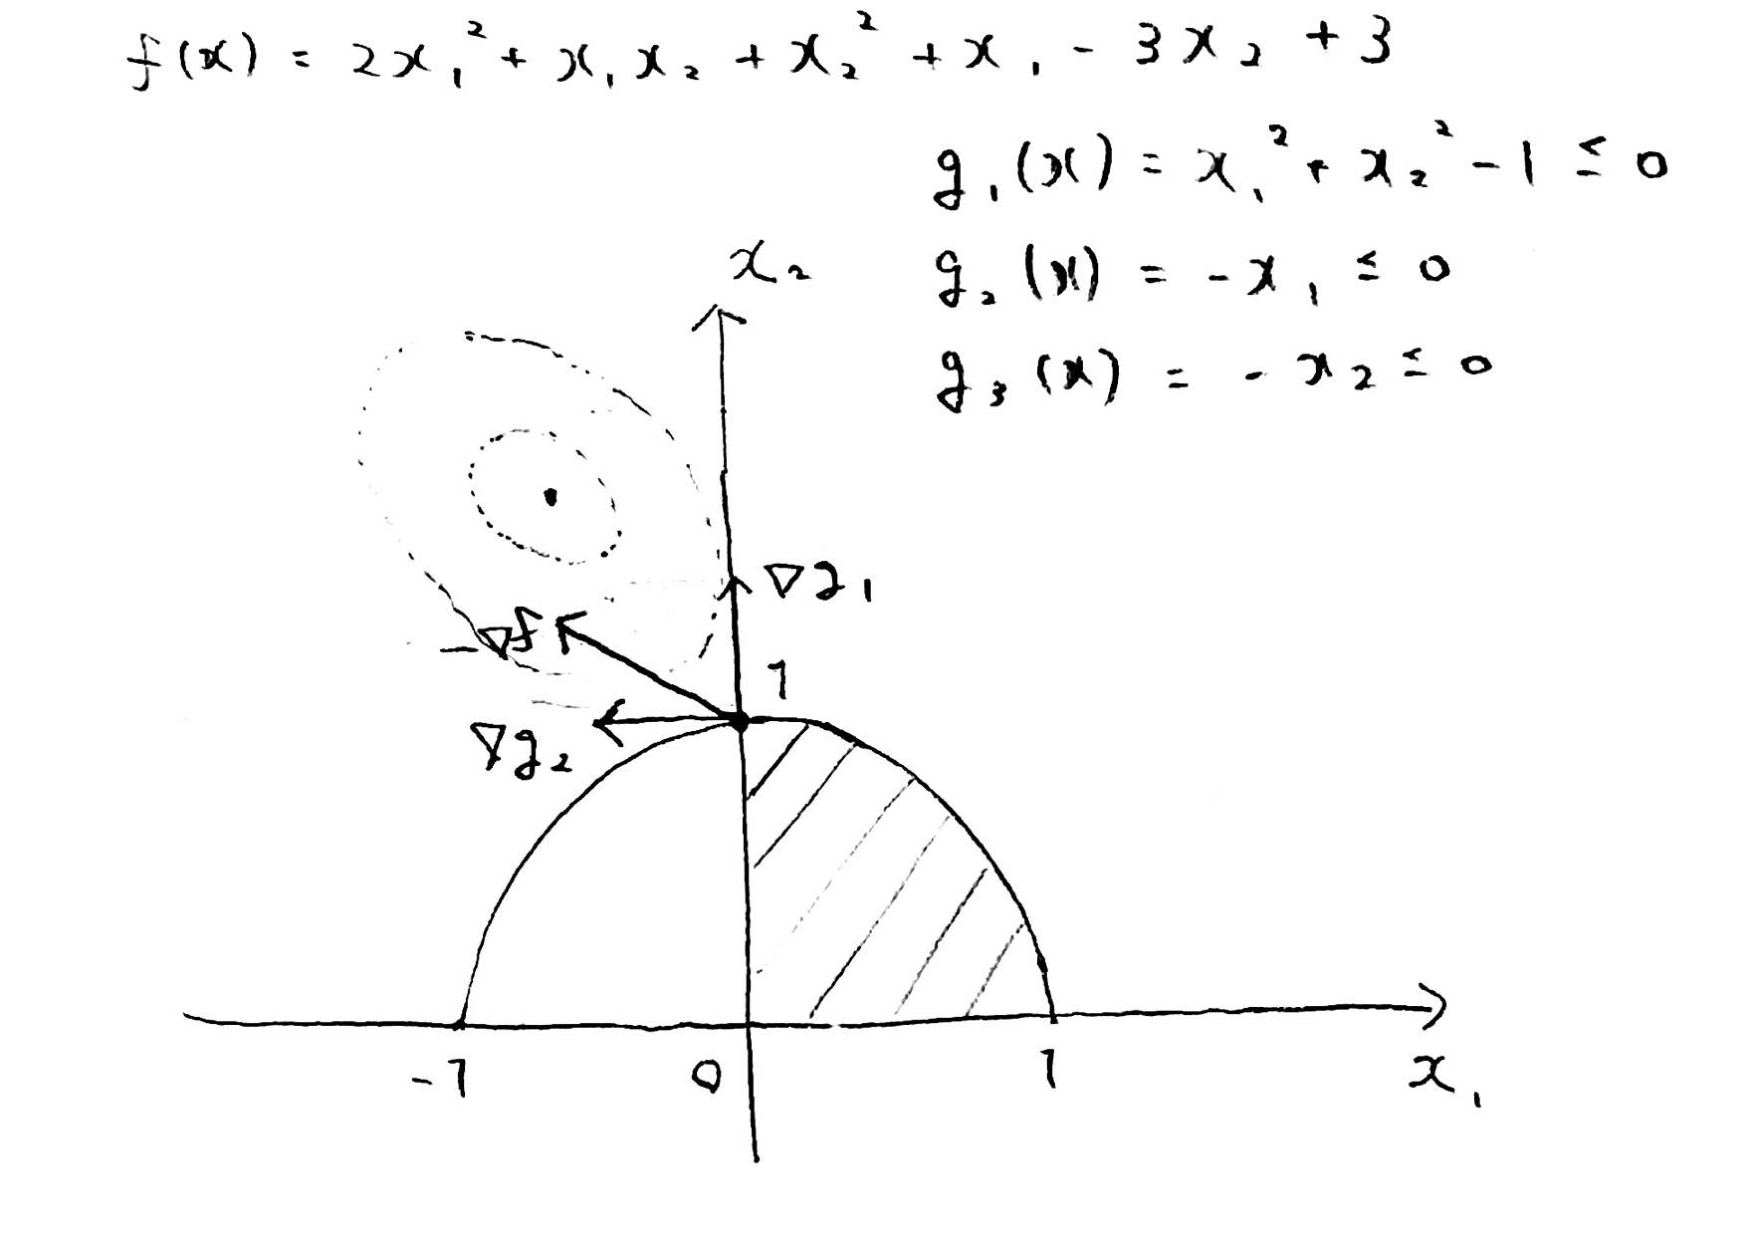
\includegraphics[clip, width=7cm]{../figure/KKT_2.pdf}
  \caption{KKT条件の幾何学的説明}
  \label{fig:KKT}
\end{figure}
$\nabla g_i(\bar{\bm{x}})$は,$\bar{\bm{x}}$における$g_i(\bm{x})$の増加方向を示す.これは,有効制約$g_i(\bm{x}) = 0$の$\bar{\bm{x}}$における接線と直交する.
また,$\nabla f(\bar{\bm{x}})$は,$\bar{\bm{x}}$における$f(\bm{x})$の増加方向を示す.$f(\bm{x})$を最小化するためには,逆方向$-\nabla f(\bm{x})$に進むのが望ましい.$-\nabla f(\bm{x})$と鋭角をなす方向へ進むことができれば,目的関数値は減少する.

$\nabla g_i(\bar{\bm{x}})$を,非負の重み$u_i \geq 0$によって加えたベクトルの領域
\begin{equation}
  G(\bar{\bm{x}}) = \{u_1 \nabla g_1(\bar{\bm{x}}) + u_2 \nabla g_2(\bar{\bm{x}}) \, | \, u_1 \geq 0, u_2 \geq 0\} \nonumber
\end{equation}
を定義する.

KKT条件は,ベクトル$-\nabla f(\bar{\bm{x}})$がこの領域内に入ることを要求している.つまり,この条件は,$\bar{\bm{x}}$から実行可能領域のどの方向を選んでも$-\nabla f(\bar{\bm{x}})$と鋭角をなすことができず,目的関数値を減少させることができないことを表す.つまり,$\bar{\bm{x}}$の局所最適性の必要条件となっている.

\section{凸計画問題}\label{sec:convex_prob}
最適化問題(\ref{eq:opt})において,実行可能領域$S \cap X$が凸集合であり,目的関数$f$が凸関数であるものを凸計画問題という.凸計画問題に対して,次の定理が成立する.
\begin{theo}\label{theo:convex_problem}
  最適化問題
  \begin{align}
    \mathrm{minimize} \; \; &f(\bm{x}) \nonumber\\
    \mathrm{subject \; to} \; \; &\bm{x} \in S \cap X \nonumber
  \end{align}
  が凸計画問題であれば,任意の局所最適解は大域最適解である.さらに,目的関数$f$が狭義凸関数のとき,大域最適解が存在すれば唯一である.
\end{theo}

線形計画問題は,実行可能領域が凸多面体であり,目的関数が凸関数であるため,凸計画問題である.非線形計画問題について,実行可能領域が
\begin{equation}\label{eq:feasible_region}
  S = \{\bm{x} \in \mathbb{R}^n \, | \, g_i(\bm{x}) \leq 0, \, i = 1, 2, \ldots, m\}
\end{equation}
である場合を考える.このとき,$g_i(\bm{x})$が凸関数であれば,
\begin{equation}
  g_i(\bm{x}) \leq 0 \nonumber
\end{equation}
を満たす$\bm{x}$の領域は凸集合である\footnote{この条件を満たす任意の2点$\bm{x}^1, \bm{x}^2$を結ぶ線分上の点$\bm{x}_{\alpha} = (1 - \alpha)\bm{x}^1 + \alpha \bm{x}^2$
は,$g_i$の凸性より,
\begin{equation}
  g_i(\bm{x}_{\alpha}) = g_i((1 - \alpha)\bm{x}^1 + \alpha \bm{x}^2) \leq (1 - \alpha)g_i(\bm{x}^1) + \alpha g_i(\bm{x}^2) \leq 0 \nonumber
\end{equation}
を満たす.補題\ref{lemm:convex}より,(\ref{eq:feasible_region})は凸集合である.\qed
}.

等式制約$g_i(\bm{x}) = 0$は,$g_i(\bm{x}) \leq 0$と$-g_i(\bm{x}) \leq 0$を合わせたものである.$g_i(\bm{x})$と$-g_i(\bm{x})$がともに凸関数であるのは,1次式$g_i(\bm{x}) = \bm{a}^{\mathrm{T}}\bm{x} - b$に限る.
\end{document}
